\textbf{{1.进程的3种基本状态}}

\textbf{就绪状态:}进程已获得了除处理器以外的所有资源,一旦获得处理器,就可以立即执行,此时进程所处的状态为就绪状态。

\textbf{执行状态(运行状态):}当一个进程获得必要的资源并正在CPU上执行时,该进程所处的状态为执行状态。

\textbf{阻塞状态(等待状态):}正在执行的进程,由于发生某事件而暂时无法执行下去(如等待I/O完成),此时进程所处的状态为阻塞状态。当进程处于阻塞状态时,即使把处理器分配给该进程,它也无法运行。

\textbf{{2.进程状态的相互转换}}\\

下图给出了进程的3种基本状态以及引起状态转换的典型原因。

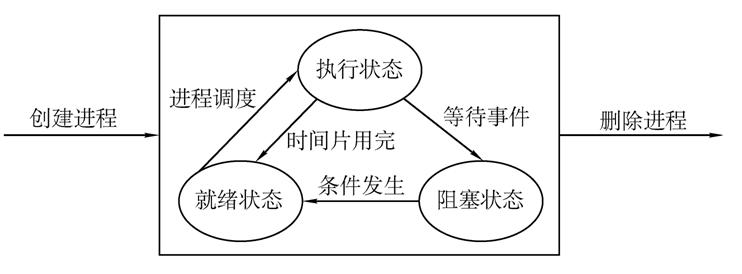
\includegraphics[width=3.33333in,height=1.22917in]{png-jpeg-pics/57AEB4CE7E8D38FE0EB467C74A138DAF.png}

\textbf{a.} \textbf{就绪状态→执行状态:}一个进程被进程调度程序选中。\\
\textbf{b. 执行状态→阻塞状态:}请求并等待某个事件发生。\\
\textbf{c.
执行状态→就绪状态:}时间片用完或在抢占式调度中有更高优先级的进程变为就绪状态。\\
\textbf{d. 阻塞状态→就绪状态:}进程因为等待的某个条件发生而被唤醒。
